%\documentclass[12pt,notitlepage]{article}
\documentclass[a4paper,12pt]{article}
\usepackage[utf8]{inputenc}
\usepackage{graphicx}
\usepackage{verbatim}
\usepackage{amsthm}
\usepackage{pdfpages}
\usepackage{amsmath}

\usepackage{mathtools}
\DeclarePairedDelimiter\ceil{\lceil}{\rceil}
\DeclarePairedDelimiter\floor{\lfloor}{\rfloor}

\usepackage{hyperref}
%\usepackage[T1]{fontenc}
\usepackage{url}
\usepackage{lipsum}
\usepackage{array}
\usepackage{multirow}
\usepackage{float}
\usepackage{lscape}
\usepackage{colortbl}
\newcolumntype{P}[1]{>{\centering\arraybackslash}p{#1}}
\usepackage[nottoc,numbib]{tocbibind}
\usepackage{fancyhdr}
\usepackage{hhline}
\usepackage[printonlyused]{acronym}

%\usepackage{txfonts}
\usepackage{lipsum,etoolbox}% http://ctan.org/pkg/{lipsum,etoolbox}
\usepackage{caption}
\usepackage{subcaption}

\usepackage{algorithm}
\usepackage[noend]{algpseudocode}

\makeatletter
\def\BState{\State\hskip-\ALG@thistlm}
\makeatother

\usepackage{minted}

\definecolor{black}{RGB}{0,0,0}

\usepackage{fancyvrb}

\usepackage{geometry}
\geometry{
	a4paper,
	total={170mm,257mm},
	right=3cm,
	left=3.5cm,
	top=3cm,
	bottom=3cm
}


\usepackage{titlesec}
\usepackage{hyperref}
\titleclass{\subsubsubsection}{straight}[\subsection]

\newcounter{subsubsubsection}[subsubsection]
\renewcommand\thesubsubsubsection{\thesubsubsection.\arabic{subsubsubsection}}
\renewcommand\theparagraph{\thesubsubsubsection.\arabic{paragraph}} % optional; useful if paragraphs are to be numbered

\titleformat{\subsubsubsection}
{\normalfont\normalsize\bfseries}{\thesubsubsubsection}{1em}{}
\titlespacing*{\subsubsubsection}
{0pt}{3.25ex plus 1ex minus .2ex}{1.5ex plus .2ex}

\makeatletter
\renewcommand\paragraph{\@startsection{paragraph}{5}{\z@}%
	{3.25ex \@plus1ex \@minus.2ex}%
	{-1em}%
	{\normalfont\normalsize\bfseries}}
\renewcommand\subparagraph{\@startsection{subparagraph}{6}{\parindent}%
	{3.25ex \@plus1ex \@minus .2ex}%
	{-1em}%
	{\normalfont\normalsize\bfseries}}
\def\toclevel@subsubsubsection{4}
\def\toclevel@paragraph{5}
\def\toclevel@paragraph{6}
\def\l@subsubsubsection{\@dottedtocline{4}{7em}{4em}}
\def\l@paragraph{\@dottedtocline{5}{10em}{5em}}
\def\l@subparagraph{\@dottedtocline{6}{14em}{6em}}
\makeatother
\usepackage{tikz}

\newcommand*\circled[1]{\tikz[baseline=(char.base)]{
		\node[shape=circle,draw,inner sep=2pt] (char) {#1};}}


\setcounter{secnumdepth}{4}
\setcounter{tocdepth}{4}

\begin{document}
	\begin{titlepage}
		\begin{center}
			\includegraphics[width = \textwidth]{logo_ntu_new.png}
			\vspace*{3cm}
			
			\Large
			\textbf{MH1401: Algorithms \& Computing I\\ Python Crash Course}\\		
			\vspace{1.5cm}
			\textbf{By\\ Brandon Goh Wen Heng}\\
			\vspace{1.5cm}November 2017\\\vspace{1.5cm}
			Mathematical Sciences\\
			\vfill
		\end{center}
	\end{titlepage}

\pagenumbering{roman}

	\tableofcontents
	\newpage
\phantomsection
\addcontentsline{toc}{section}{About}
\section*{About}
{\par \noindent This document will go through common mistakes and things to take note when programming for PYTHON and should be helpful for your exam and future modules.}
\newpage
\pagenumbering{arabic}
\addcontentsline{toc}{section}{Things To Take Note}
\section*{Things To Take Note}
\circled{0} \textbf{IMPORTANT}\\\\
\circled{1} \textbf{Structure of Python Script}\\

\newpage
\subsection*{\circled{0} IMPORTANT}
\vspace{1em}
{\par \noindent Take note that just because your program works \textbf{\underline{DOES NOT}} mean that it is correct and will always work on different computers and compilers.
\subsection*{\circled{1} Structure of Python Script}
\vspace{1em}
{\par \noindent The structure of the code should consist of the following:}
\begin{enumerate}
	\item Importing modules
	\item Function Declaration
	\item Script
	\end{enumerate}

\begin{figure}[H]
	\centering
	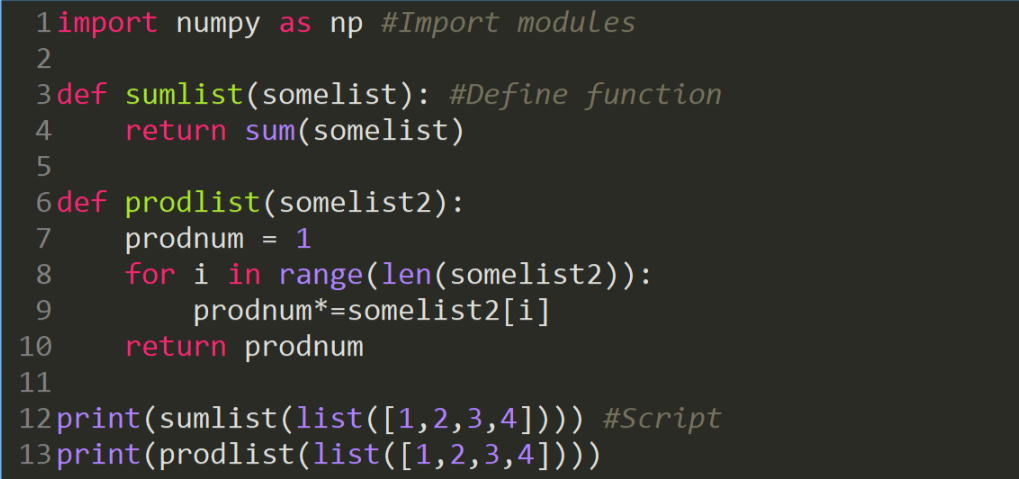
\includegraphics[width=1\linewidth]{pythonbackbone}
	\caption{Typical structure of Python code}
	\label{fig:pythonmodexcep}
\end{figure}
\subsection*{\circled{1.1} Importing Modules}
{\par Typically, modules are declared at the top of the Python file above everything else. However, in some cases there may be exceptions. In Figure 2 below, we import the module \texttt{numpy} as we will only be using it \textbf{inside} the function.}
\begin{figure}[H]
	\centering
	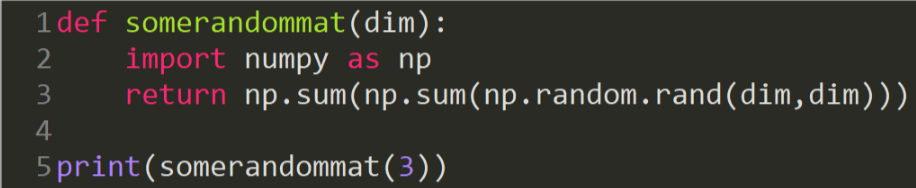
\includegraphics[width=1\linewidth]{pythonmodexcep}
	\caption{\texttt{Numpy} imported for the function only}
	\label{fig:pythonmodexcep}
\end{figure}
{\par \noindent $\star$We do not define functions in an \texttt{if, else, for, while} etc. statement. As long as it needs to be used somewhere, it should be put at the top.\\\\$\star$Do \textbf{\underline{NOT}} import every library that you can think of and not use it. It is highly inefficient and will make your program very bloated.}
\end{document}